\documentclass{article}
\usepackage[T1]{fontenc}
\usepackage{lmodern}
\usepackage[paperwidth=841mm, paperheight=594mm, margin=20mm]{geometry}
\usepackage{xcolor}
\usepackage{tikz}
\usepackage[skins]{tcolorbox}
\usepackage{pgfplots}
\usepackage{enumitem}
\usepackage{array}
\pgfplotsset{compat=1.18}

% One colour per step of the scientific method. Change freely.
\definecolor{cq}{HTML}{FF6B6B}
\definecolor{ch}{HTML}{FFA94D}
\definecolor{cm}{HTML}{FFD43B}
\definecolor{cp}{HTML}{69DB7C}
\definecolor{cr}{HTML}{4DABF7}
\definecolor{cc}{HTML}{9775FA}
\definecolor{board}{HTML}{FFF9EC}

% Text size for an A1 poster.
\newcommand{\bodysize}{\fontsize{34}{43}\selectfont}

\renewcommand{\familydefault}{\sfdefault}
\pagestyle{empty}
\setlength{\parindent}{0pt}
\setlist{leftmargin=1.1em, itemsep=4pt, topsep=4pt}

% A step card. Usage: \begin{card}{colour}{Title} ... \end{card}
\newtcolorbox{card}[2]{enhanced, colback=white, colframe=#1, boxrule=4pt, arc=10mm,
  left=8mm, right=8mm, top=6mm, bottom=6mm, before skip=0pt, after skip=10mm,
  title={#2}, fonttitle=\fontsize{42}{48}\selectfont\bfseries, coltitle=black, colbacktitle=#1,
  toptitle=2mm, bottomtitle=2mm, drop shadow={black!25}}

\begin{document}
\bodysize

\begin{tikzpicture}[remember picture, overlay]
  \fill[board] (current page.south west) rectangle (current page.north east);
\end{tikzpicture}

% Project title banner: edit the title and student details.
\begin{tcolorbox}[enhanced, colback=cr!15, colframe=cr, boxrule=5pt, arc=12mm, halign=center,
    top=8mm, bottom=8mm, after skip=12mm]
  {\fontsize{80}{88}\selectfont\bfseries Which Paper Towel Soaks Up the Most Water?\par}
  \vspace{6mm}
  {\fontsize{32}{38}\selectfont Maya Chen and Leo Park \quad Grade 7 \quad Example Middle School\par}
\end{tcolorbox}

\begin{minipage}[t]{0.29\linewidth}
  \vspace{0pt}
  \begin{card}{cq}{1. Question}
    Do more expensive paper towels really absorb more water than cheaper ones?
  \end{card}
  \begin{card}{ch}{2. Hypothesis}
    If a towel costs more, then it will absorb more water, because it is usually thicker.
  \end{card}
  \begin{card}{cm}{3. Materials}
    \begin{itemize}
      \item 4 brands of paper towel
      \item Measuring cup and scale
      \item Bowl of water, timer
      \item Notebook for results
    \end{itemize}
  \end{card}
  \begin{card}{cm}{Variables}
    \textbf{Changed:} brand of towel\\
    \textbf{Measured:} water held\\
    \textbf{Kept the same:} sheet size, dip time, drip time
  \end{card}
  \begin{card}{ch}{Did you know?}
    Paper towels hold water in tiny gaps between their fibres, a bit like a sponge.
  \end{card}
\end{minipage}\hfill
\begin{minipage}[t]{0.38\linewidth}
  \vspace{0pt}
  \begin{card}{cp}{4. Procedure}
    \begin{enumerate}
      \item Cut one sheet of each brand to the same size.
      \item Weigh the dry sheet.
      \item Dip it in water for 10 seconds.
      \item Let it drip for 30 seconds, then weigh again.
      \item Repeat 5 times for each brand.
    \end{enumerate}
  \end{card}
  \begin{card}{cr}{5. Data}
    \centering
    \renewcommand{\arraystretch}{1.3}
    % Type your own measurements into this table.
    \begin{tabular}{lcc}
      \textbf{Brand} & \textbf{Price per roll} & \textbf{Water held (g)} \\
      \hline
      A & \$0.90 & 18 \\
      B & \$1.40 & 24 \\
      C & \$2.10 & 23 \\
      D & \$2.80 & 29 \\
    \end{tabular}
  \end{card}
  \begin{card}{cr}{Photo}
    \centering
    \tikz\node[draw=gray, dashed, line width=2pt, minimum width=0.9\linewidth, minimum height=110mm]{Image placeholder};
  \end{card}
\end{minipage}\hfill
\begin{minipage}[t]{0.29\linewidth}
  \vspace{0pt}
  \begin{card}{cr}{6. Results}
    \centering
    % Change the bar heights to match your data table.
    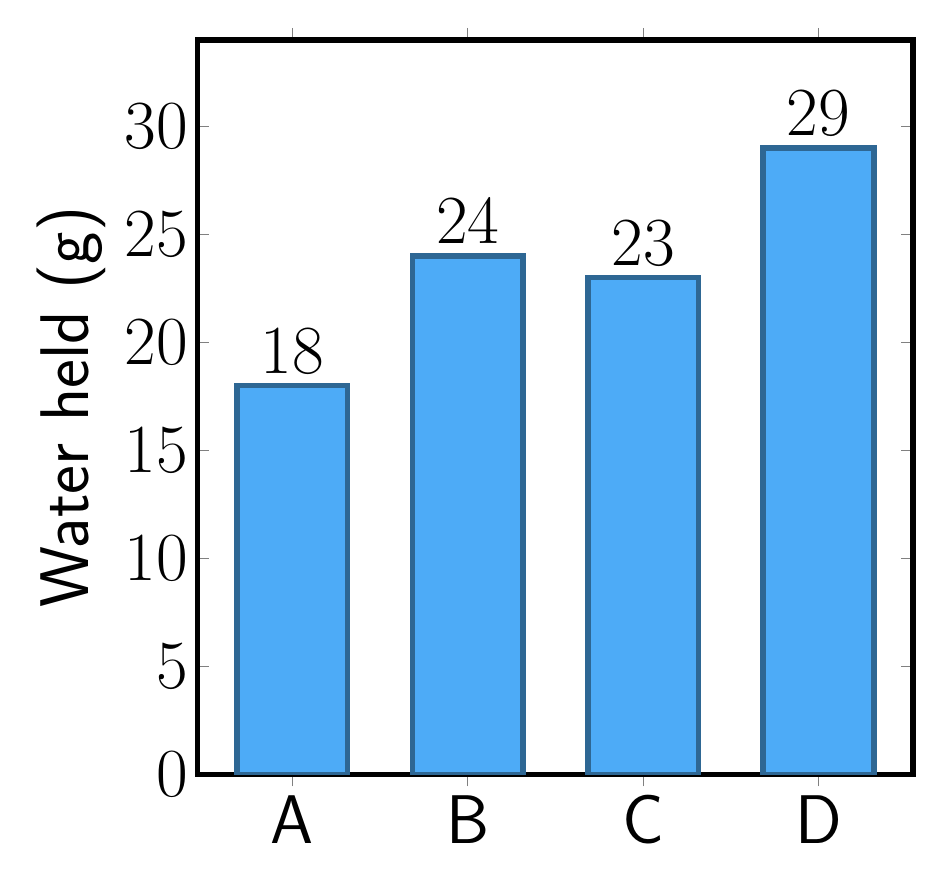
\begin{tikzpicture}
      \begin{axis}[ybar, width=0.88\linewidth, height=0.9\linewidth, bar width=40pt, enlarge x limits=0.18,
          symbolic x coords={A,B,C,D}, xtick=data, ymin=0, ymax=34, ylabel={Water held (g)},
          font=\bodysize, tick label style={font=\bodysize}, nodes near coords,
          axis line style={line width=2pt}, every node near coord/.append style={font=\bodysize}]
        \addplot[fill=cr, draw=cr!60!black, line width=2pt] coordinates {(A,18) (B,24) (C,23) (D,29)};
      \end{axis}
    \end{tikzpicture}
  \end{card}
  \begin{card}{cc}{7. Conclusion}
    Our hypothesis was \textbf{partly supported}. The most expensive towel held the most water, but brand C held less than cheaper brand B.
  \end{card}
  \begin{card}{cc}{What we would try next}
    Test towels with different textures, and use warm water.
  \end{card}
\end{minipage}

\end{document}
